%\placelogofalse
\begin{frame}{The FEniCS Project}
\begin{columns}
\column{0.58\linewidth}
\centering
\begin{outline}
  \1 Collection of opensource software 
  \1 Used to create models with FEM
  \1 Origins in 2002
  \1 Steady development / rewrites
  \1 Very popular for research
  \1 Unified Form Language (UFL) 
\end{outline}

\column{0.38\linewidth}
\begin{center}
\centering

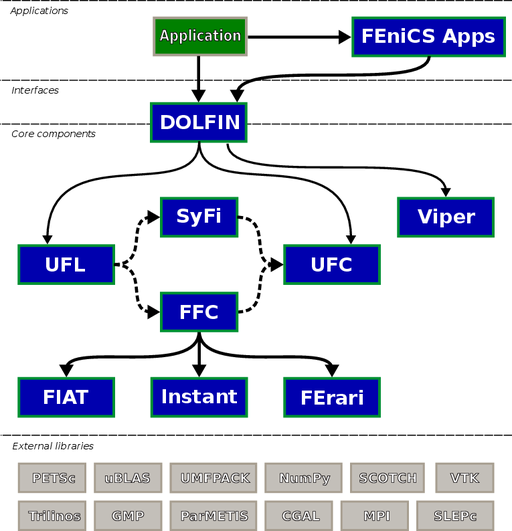
\includegraphics[width=\linewidth]{assets/Fenics-map.png}

%\shadowimage[width=2.5cm]{example_1.png}

%\includegraphics[width=2.5cm]{example_3.png}

% [trim={left bottom right top},clip]
%
\includegraphics[width=8.5cm, page=3, trim={0 9cm 14cm 0cm},clip]{assets/vec_db_figs.pdf}
\end{center}
\end{columns}
%\blfootnote{From \href{https://en.wikipedia.org/wiki/FEniCS_Project#/media/File:Fenics-map.png}{Wikipedia}}
\end{frame}
%\placelogotrue
